% -*- TeX -*- -*- UK -*- -*- BMR -*-
% ----------------------------------------------------------------
% Beamer presentation ************************************************
%
% Subhaneil Lahiri's template
%
% To compile:
%   Ctrl-Shift-P
%
% **** -----------------------------------------------------------
\documentclass{beamer}%[hyperref={backref=slide}]

%\input{sl_slide_preamble.tex}
\input{sl_slide_preamble_nonotes.tex}
\input{sl_slide_graphics_preamble.tex}
\input{sl_definitions.tex}
\input{sl_slide_symbols.tex}
%
\usecolortheme[rgb={0.37843137 0.07058824 0.5372549}]{structure}
%
\graphicspath{{"Figures/"}}
%matrices
\newcommand{\inv}{^{-1}}
\newcommand{\I}{\mathbf{I}}
%prob vector
\newcommand{\pr}{\mathbf{p}}
%equilibrium distribution
\newcommand{\eq}{\pr^\infty}
%first passage times
\newcommand{\fpt}{\mathbf{T}}
%off-diag first passage times
\newcommand{\fptb}{\overline{\fpt}}
%other symbols
\newcommand{\w}{\mathbf{w}}
\newcommand{\W}{\mathbf{W}}
\newcommand{\frg}{\W^\mathrm{F}}
\newcommand{\M}{\mathbf{M}}
\newcommand{\F}{\boldsymbol{\Phi}}
%\newcommand{\wv}{\vec{w}}
%snr curves etc
\newcommand{\syn}{\vec{w}}
\newcommand{\synid}{\syn_\text{ideal}}
\DeclareMathOperator{\SNR}{SNR}
\DeclareMathOperator{\snr}{SNR}
\newcommand{\snrb}{\overline{\snr}}
%super/subscripts
\newcommand{\pot}{^{\text{pot}}}
\newcommand{\dep}{^{\text{dep}}}
\newcommand{\potdep}{^{\text{pot/dep}}}
\newcommand{\lmax}{_{\text{max}}}
\newcommand{\lmin}{_{\text{min}}}
%quantities
\newcommand{\initial}{\mathcal{I}}
\newcommand{\area}{\mathcal{A}}
\newcommand{\CS}{\mathcal{S}}
\newcommand{\comp}{^\mathrm{c}}
\renewcommand{\e}{\mathsf{e}}
%---------Title-----------------------------------------------------------

\title[Complex synapses]{Learning and memory with complex synaptic plasticity}
%
\subtitle{\small{based on work with Surya Ganguli}
}
%
\author{Subhaneil Lahiri%\inst{1}
}
%
\institute[Stanford]{%
%\inst{1}
Stanford University, Applied Physics
}
%
%\slideCaption{}

%---------Beginning--------------------------------------------------------

\begin{document}

%-------------Slide--------------------------------------------------------

\begin{frame}
%
 \titlepage
%
\end{frame}

%-------------Slide--------------------------------------------------------

\begin{frame}{Introduction}
%
 We often model synaptic plasticity as the change of a single number (synaptic weight).
 %
 \note[item]{amplitude of psp.}
 %
 In reality, there is a complex dynamical system inside a synapse.

 \vp Semi-realistic models of synaptic plasticity have terrible memory without synaptic complexity.
 %
 \note[item]{finite number of values.}

 \vp We will study the entire space of a broad class of models of complex synapses to find upper bounds on their performance.

 \vp This leads to understanding of what structures are useful for storing memories for different timescales.
%
\end{frame}

%-------------Slide--------------------------------------------------------

\begin{frame}{Synaptic learning and memory}
%
% \textbf{Learning rule:} how activity $\to$ potentiation/depression.\\
% \hp \eg Hebb rule, STDP, Hopfield outer product, perceptron rule,\ldots
%
% \vp \textbf{Plasticity mechanism:} how synapse responds to potentiation/depression.\\
% \hp \eg Binary switch, Cascade model, Multistate model,\ldots
%
% \vp \textbf{Memory retrieval:} how synaptic state affects neural activity.\\
% \hp \eg Hopfield attractor,\ldots
 \begin{center}
  \only<1>{\includegraphics[width=0.7\linewidth]{synaptic_learning0.svg}}%
  \only<2>{\includegraphics[width=0.7\linewidth]{synaptic_learning.svg}}%
 \end{center}

 \note[item]{Avoid confusion: separate concepts}
 \note[item]{Talk exclusively about second one.}
 \note[item]{Abstract away other two.}
%
\end{frame}

%-------------Slide--------------------------------------------------------

\begin{frame}[label=fr_net]{Synapses are complex}
%
 \parbox[t]{0.45\linewidth}{%
 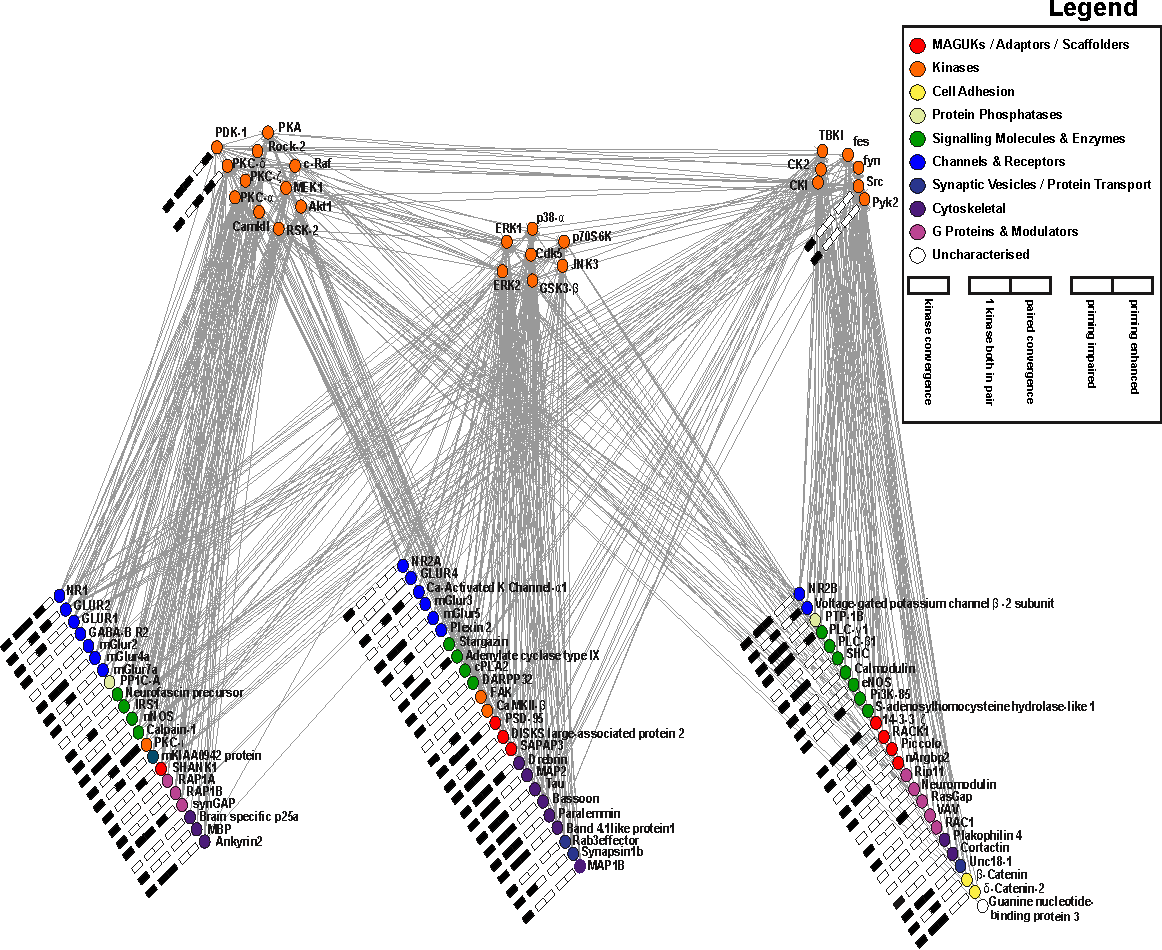
\includegraphics[height=0.8\linewidth]{2000102CobaFig4.pdf}

 \citerr{Coba2009phosphorylation}
 }
 \hspace{0.05\linewidth}
 \parbox[t]{0.45\linewidth}{%
 \hfill
 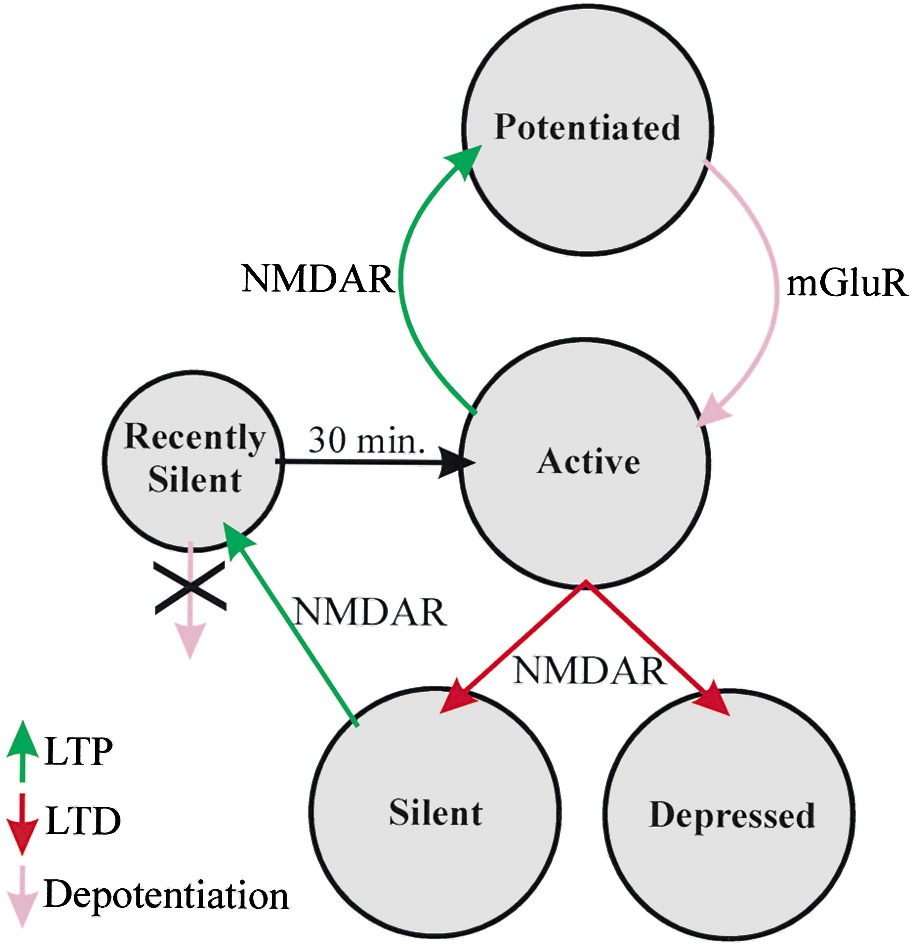
\includegraphics[height=0.8\linewidth]{MadisonMontgomery.jpg}

 \citerr{Montgomery2002765}
 }
 %
 \note[item]{Molecular network, post-synaptic density, from Seth Grant}
 \note[item]{Functional e-phys states from Montgomery and Madison}

 \vp\hyperlink{fr_questions}{There} is a complex, dynamic system underlying synaptic plasticity.
 %
 \note[item]{Does this matter?}
 \note[item]{Could just be the machinery for changing synaptic weight}
 \note[item]{link back to questions on ``There''}
%
\end{frame}


%-------------Slide--------------------------------------------------------

\begin{frame}{Timescales of memory}
%
 \parbox[t]{0.47\linewidth}{
 Memories stored in different places for different timescales
 \begin{center}
   \aligntop{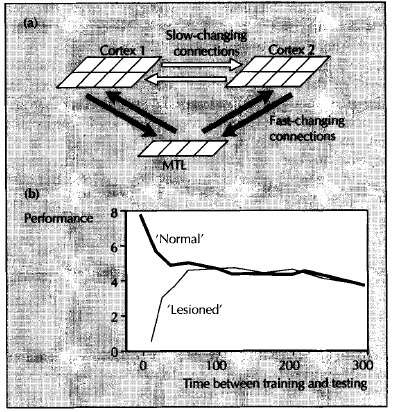
\includegraphics[width=0.4\linewidth]{SquireAlvarez.jpg}}
 \end{center}
 \citerr{Squire1995amnesia}

 \cf Cerebellar cortex vs.\ cerebellar nuclei.

 \citerr{Krakauer2006motorcons}
 }
 %
 \hspace{0.03\linewidth}
 %
 \parbox[t]{0.47\linewidth}{
 Different synapses have different molecular structures.
 \begin{center}
   \aligntop{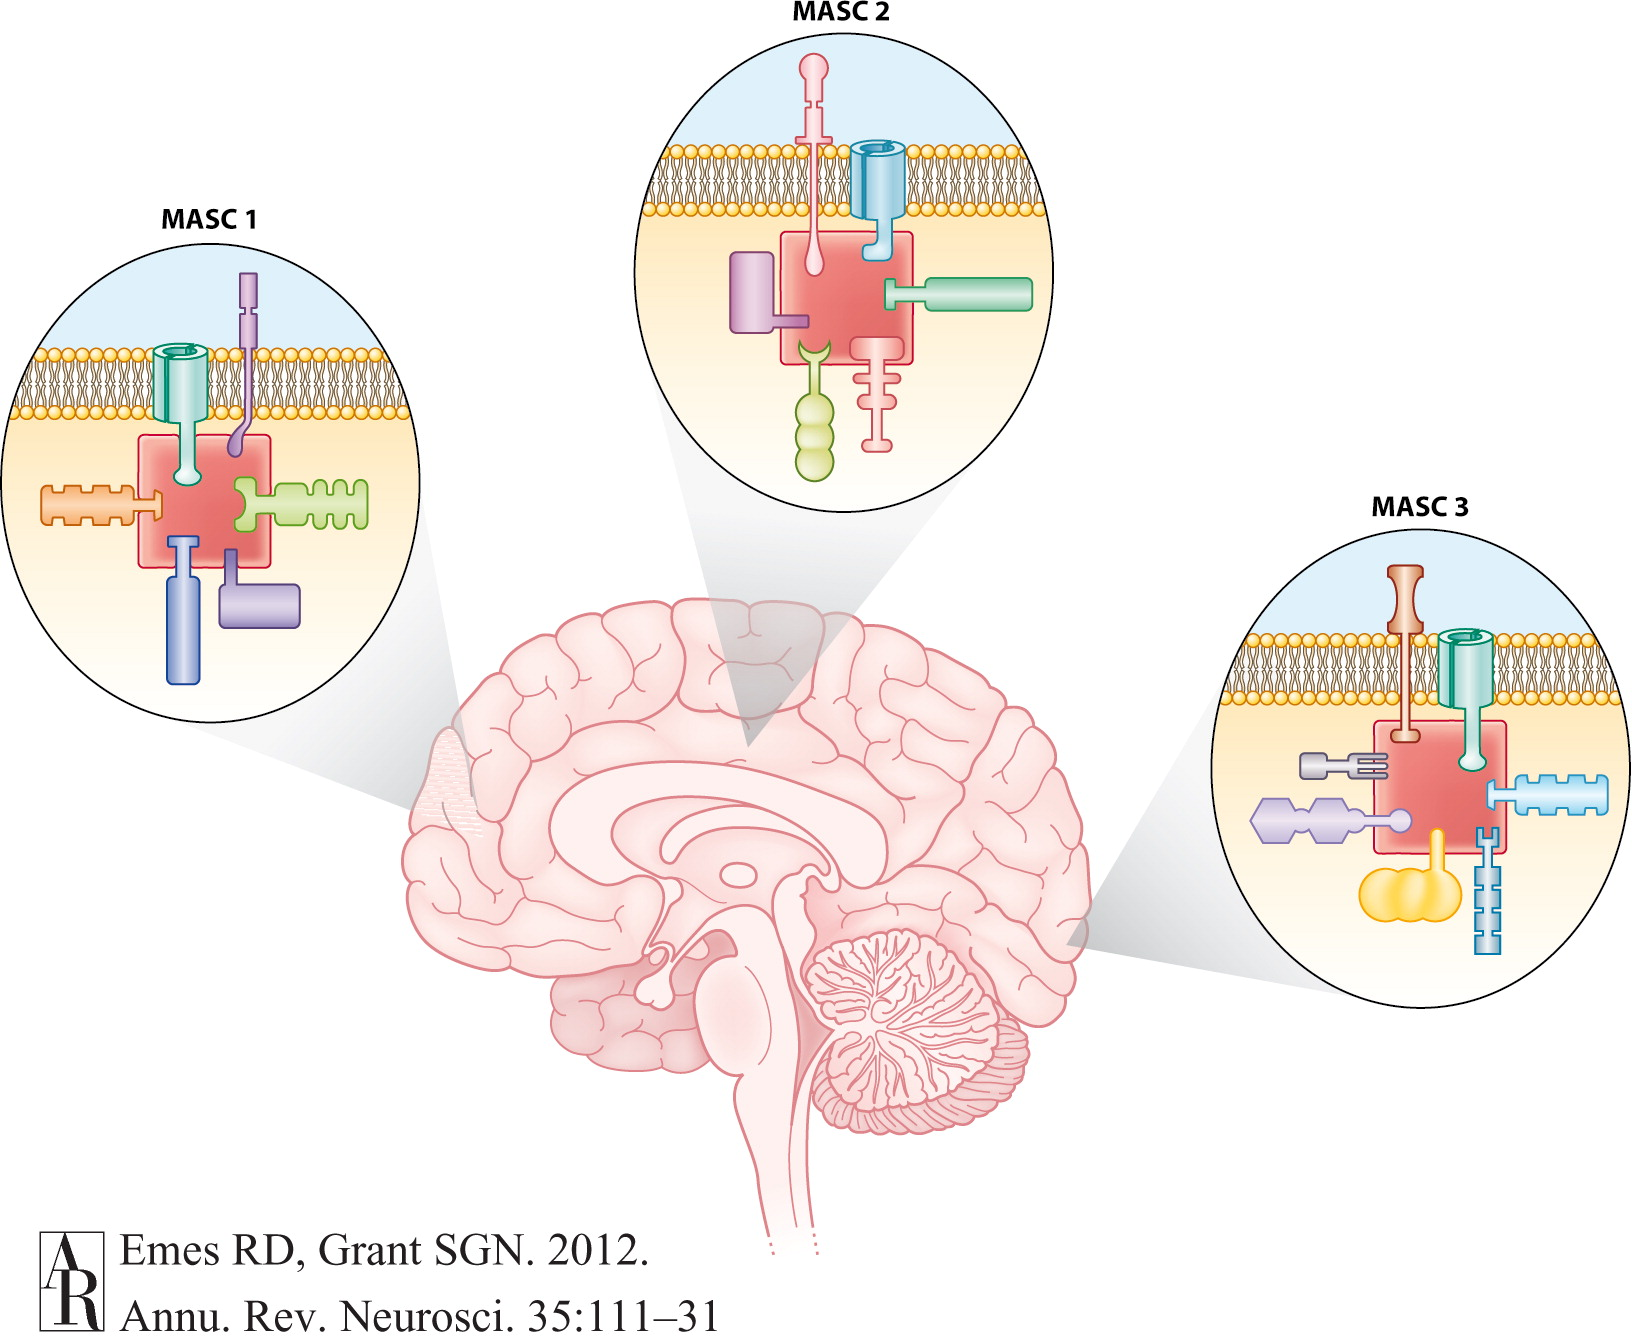
\includegraphics[width=0.6\linewidth]{Emes2012.jpeg}}
 \end{center}
 \citerr{Emes2012synapserev}
 }
 %
%
\end{frame}

%-------------Slide--------------------------------------------------------

\begin{frame}{Outline}
%
 \tableofcontents[hideallsubsections]
 %
 \note[item]{review terrible properties of simple synapses.}
 \note[item]{mathematical formalism of model, quantify performance (memory decay over time)}
 \note[item]{upper bounds on single numbers that depend on whole memory curve (decay over time)}
 \note[item]{upper bounds at finite times}
%
\end{frame}

%-------------Section--------------------------------------------------------

\section{Why complex synapses?}

%-------------Slide--------------------------------------------------------

\begin{frame}{Storage capacity of synaptic memory}
%
  A classical perceptron has a capacity $\propto N$, (\# synapses).

\vp\parbox[t]{0.59\linewidth}{%
  Requires synapses' dynamic range also $\propto N$.

 \vp With discrete, finite synapses:\\
 \hp $\implies$ new memories overwrite old.
 %
 }
 %
 \parbox[t]{0.4\linewidth}{
   %\begin{flushright}
    \hfill\aligntop{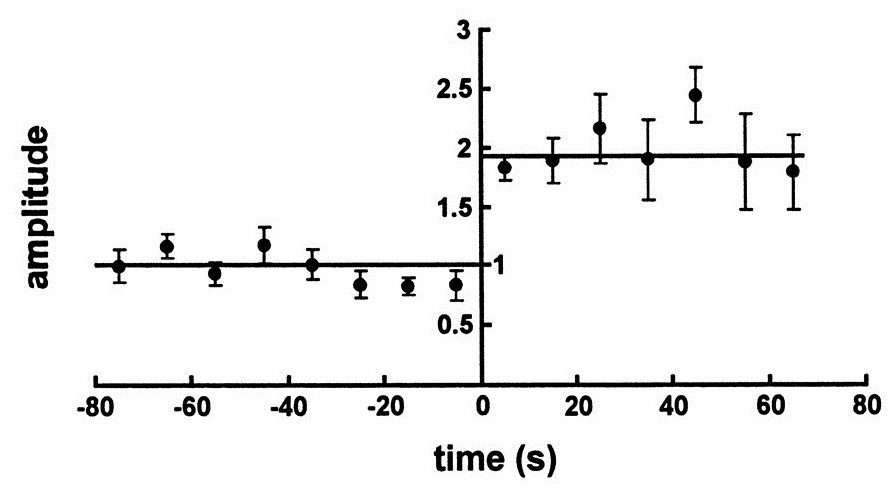
\includegraphics[width=0.9\linewidth]{Petersen1998.jpg}}
   %\end{flushright}
 }
 \\
    \citerr{Petersen1998allornone,O'Connor2005switch}

 \vp When we store new memories rapidly, memory capacity  $\sim\CO(\log N)$.
 \\ \citerr{amit1992constraints,amit1994learning}
 %
 \note[item]{or sparse $\sim \log N / N$}
%
\end{frame}


%-------------Slide--------------------------------------------------------

\begin{frame}{Trade-off between learning and remembering}
%
 {}
 \begin{center}
 \begin{tabular}{ccc}
   % after \\: \hline or \cline{col1-col2} \cline{col3-col4} ...
                & \textbf{Learning} & \textbf{Remembering} \\[0.5cm]
   \visible<1->{Very plastic} & \visible<1->{\alignmid{
\includegraphics[width=0.1\linewidth]{Face-smile.svg}}} & \visible<2->{\alignmid{
\includegraphics[width=0.1\linewidth]{Face-sad.svg}}} \\[1cm]
   \visible<3->{Very rigid}   & \visible<4->{\alignmid{
\includegraphics[width=0.1\linewidth]{Face-sad.svg}}} & \visible<3->{\alignmid{
\includegraphics[width=0.1\linewidth]{Face-smile.svg}}} \\
 \end{tabular}
 \end{center}
 \note[item]{very plastic: learn easy, forget easy}
 \note[item]{little plasticity, remember better, learn harder}

 \vp \visible<4->{Circumvent tradeoff: go beyond model of synapse as single number.}
 \note[item]{one way around limit: complexity}
%
\end{frame}


%-------------Section--------------------------------------------------------

\section{Modelling synaptic memory}

%%-------------Slide--------------------------------------------------------
%
%\begin{frame}{Complex synapses}
%%
%  \aligntop{\includegraphics[width=5cm]{synapse.svg}}\hp
%  %
%  \note[item]{functional states, not molecules}
%  \note[item]{synaptic weight depends on state}
%  \note[item]{many states can have same weight}
%  %
%  \hp\aligntop{\includegraphics[width=2cm]{pot.svg}}
%  \hp\aligntop{\includegraphics[width=2cm]{dep.svg}}
%  %
%  \note[item]{stochastic transitions}
%%
%\end{frame}
%
%-------------Slide--------------------------------------------------------

\begin{frame}{Recognition memory}
%
 Synapses given a sequence of patterns (pot \& dep) to store

 \vp
 \begin{center}
 \only<1>{\aligntop{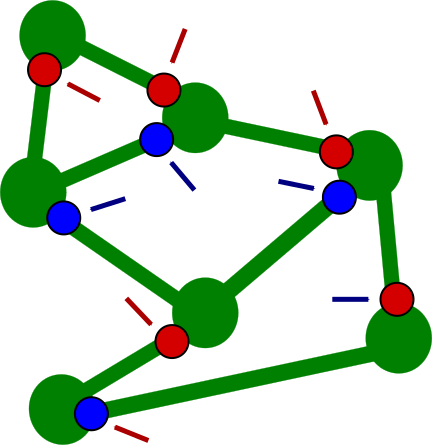
\includegraphics[width=0.35\linewidth]{network1.svg}}}%
 \only<2>{\aligntop{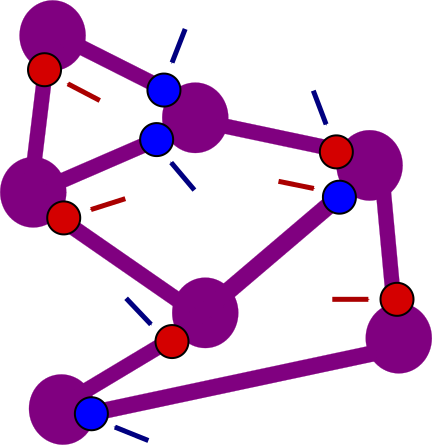
\includegraphics[width=0.35\linewidth]{network2.svg}}}%
 \only<3>{\aligntop{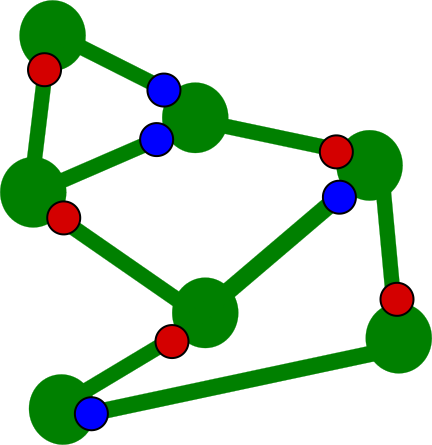
\includegraphics[width=0.35\linewidth]{network3.svg}}}%
 \only<4>{\aligntop{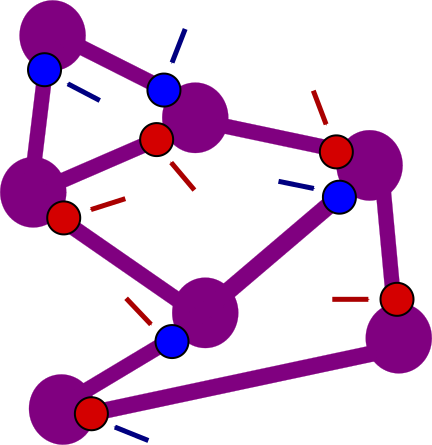
\includegraphics[width=0.35\linewidth]{network4.svg}}}%
 \only<5>{\aligntop{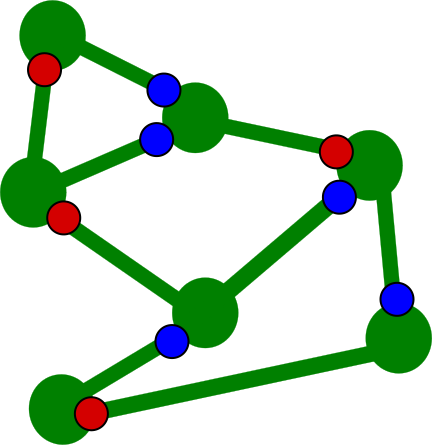
\includegraphics[width=0.35\linewidth]{network5.svg}}}%
 \only<6>{\aligntop{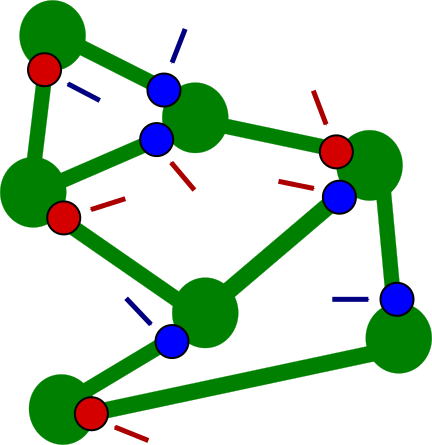
\includegraphics[width=0.35\linewidth]{network6.svg}}}%
 \only<7>{\aligntop{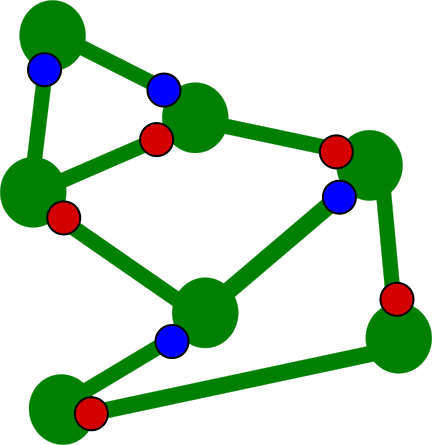
\includegraphics[width=0.35\linewidth]{network7.svg}}}%
 \only<8>{\aligntop{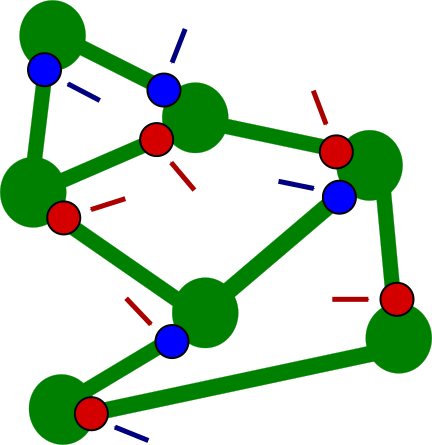
\includegraphics[width=0.35\linewidth]{network8.svg}}}%
 \end{center}

 \vp \visible<8>{Later: presented with a pattern.
 Has it been seen before?}
%

%
\end{frame}

%-------------Slide--------------------------------------------------------

\begin{frame}{Quantifying memory quality}
%
 Have we seen pattern before?
 Test if $\synid \cdot \syn(t) \gtrless \theta$?

 $\synid \cdot \syn(\infty) \sim$  null distribution
 $\implies$ ROC curve:

 \vp
 %
 \parbox[t]{0.4\linewidth}{%
 \aligntop{\includegraphics[width=0.9\linewidth]{roc.svg}}
 }
 %
 \parbox[t]{0.55\linewidth}{%
 \vspace{-\baselineskip}
 \begin{equation*}
   \begin{aligned}
%   \operatorname{TPR} &= \Phi \prn{ \frac{ \snr(t) +\Phi\inv(\operatorname{FPR}) }{ \operatorname{NNR}(t) } }, \\[0.5cm]
   %\quad\text{where } \quad
     %\Phi(x) &= \int_{-\infty}^x \frac{ \e^{-\frac{z^2}{2}} }{ \sqrt{2\pi} }\, \dr z, \\
     \snr(t) &= \frac{ \av{\synid\cdt\syn(t)} - \av{\synid\cdt\syn(\infty)} }{ \sqrt{\var(\synid\cdt\syn(\infty))}}, \\[1cm]
    \color{darkgrey} \operatorname{NNR}(t) &= \color{darkgrey} \sqrt{\frac{ \var(\synid\cdt\syn(t)) }{ \var(\synid\cdt\syn(\infty)) }}.
   \end{aligned}
 \end{equation*}
 }

%
\end{frame}

%-------------Slide--------------------------------------------------------

\begin{frame}{Averaging over recall times}
%
 Look at:
 %
 \begin{equation*}
   \qquad
   \snrb(\tau) = \av{\snr(t)}_{P\cond{t}{\tau}},
   \qquad
   P\cond{t}{\tau} = \frac{\e^{-t/\tau}}{\tau}.
 \end{equation*}
 %
 $\tau=$ mean recall time.
 
 \vp Like a ``running average'':
 %
 \begin{equation*}
   \widehat{\SNR}(\tau) = \frac{1}{\tau}\intd[_0^\infty]{t}\e^{-t/\tau}\,\SNR(t)
     \sim \frac{1}{\tau}\intd[_0^\tau]{t}\SNR(t)
 \end{equation*}
 %
 
 \vp Different brain regions \lto\ different $\tau$.
%
\end{frame}

%-------------Slide--------------------------------------------------------

\begin{frame}{Models of complex synaptic dynamics}
%
%  There are $N$ identical synapses with $M$ internal functional states.
\visible<2->{
\parbox[c]{0.82\linewidth}{%
  \begin{itemize}
    \item Internal functional state of synapse \lto\ synaptic weight.
    \item Candidate plasticity events \lto\ transitions between states
  \end{itemize}
}\hfill
\alignmid{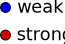
\includegraphics[width=0.13\linewidth]{state_key.svg}}
}

  %
  \vp
%  \begin{overlayarea}{0.7\linewidth}{0.3\linewidth}
%    \only<1>{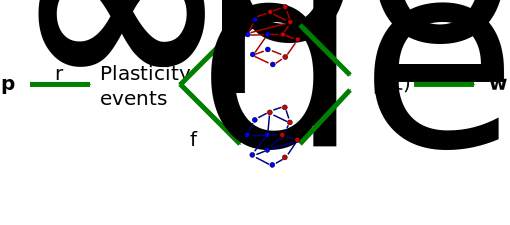
\includegraphics[width=0.99\linewidth]{synapse_model_1.svg}}%
%    \only<2>{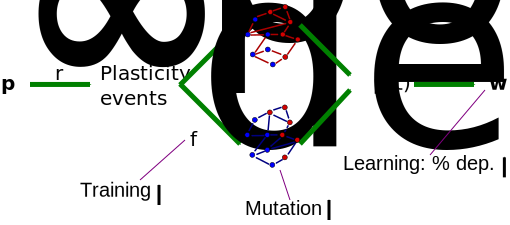
\includegraphics[width=0.99\linewidth]{synapse_model_2.svg}}
%  \end{overlayarea}
%
\begin{overlayarea}{0.95\linewidth}{0.4\textheight}
  \begin{center}
%\aligntop{\movie[width=200px,height=92px,showcontrols=true,loop]{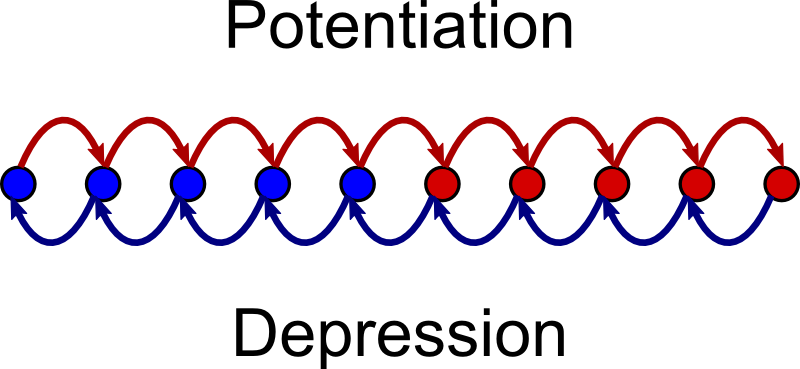
\includegraphics[width=200px,height=92px]{Vids/plast_00.png}}{plast.avi}}
    \only<1>{\aligntop{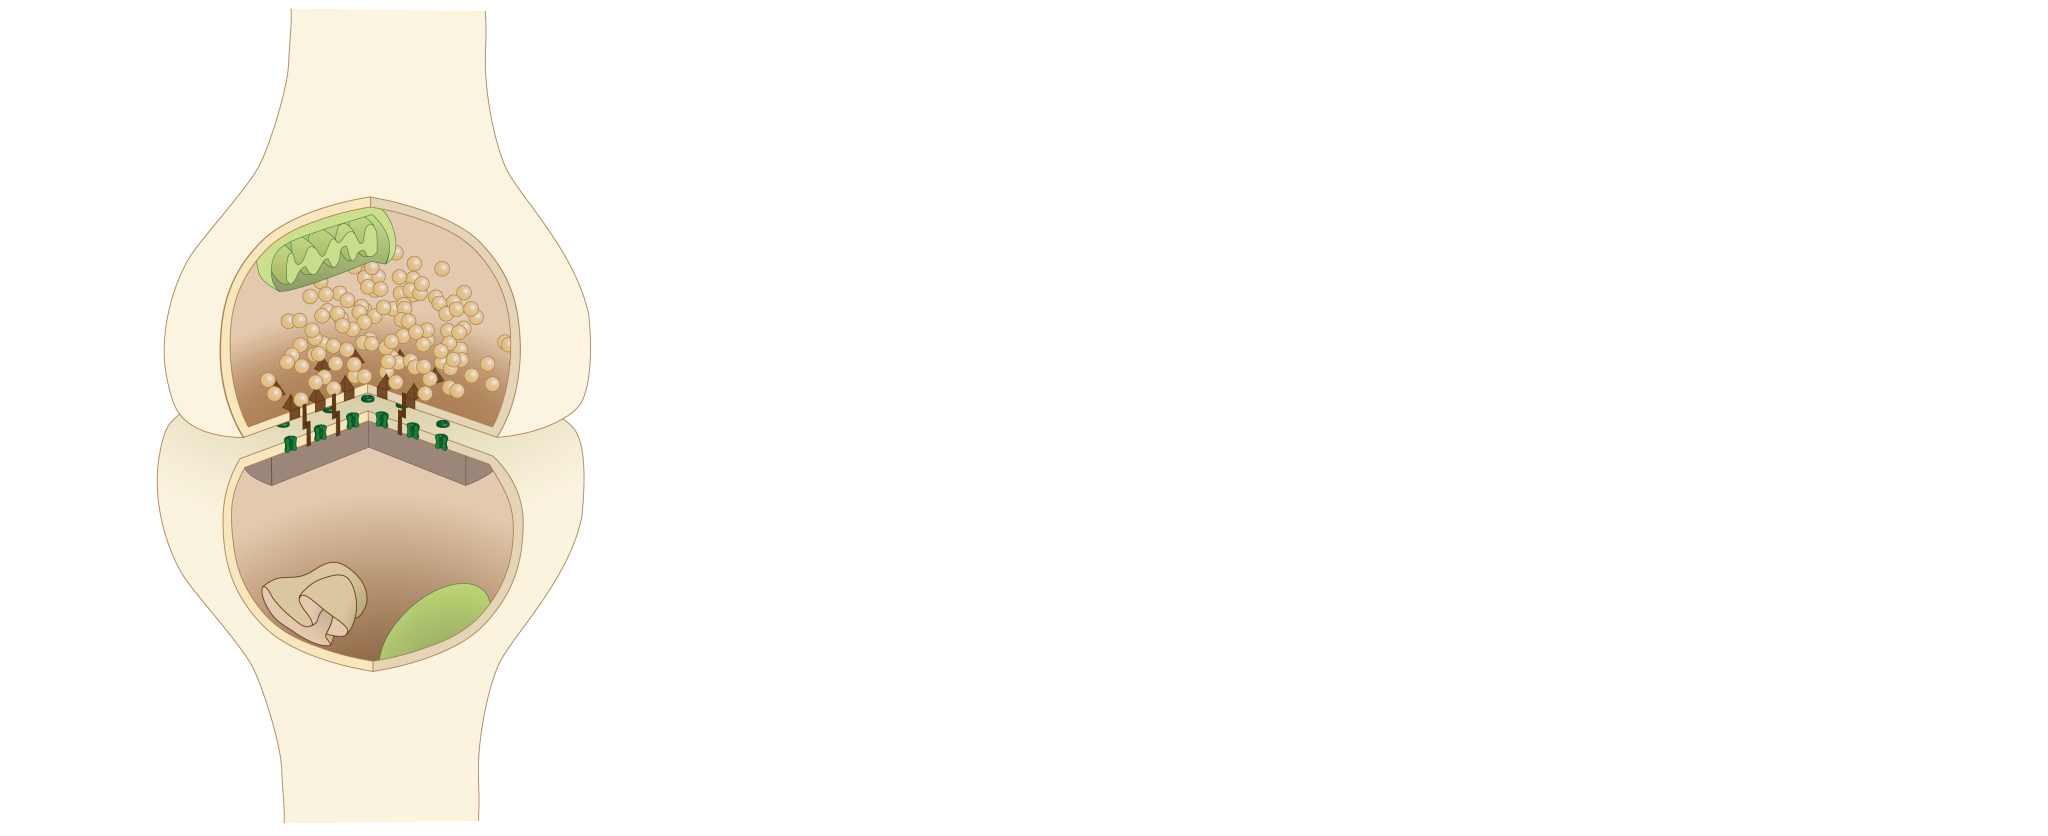
\includegraphics[width=0.7\linewidth]{serial_internal_1.svg}}}%
    \only<2>{\aligntop{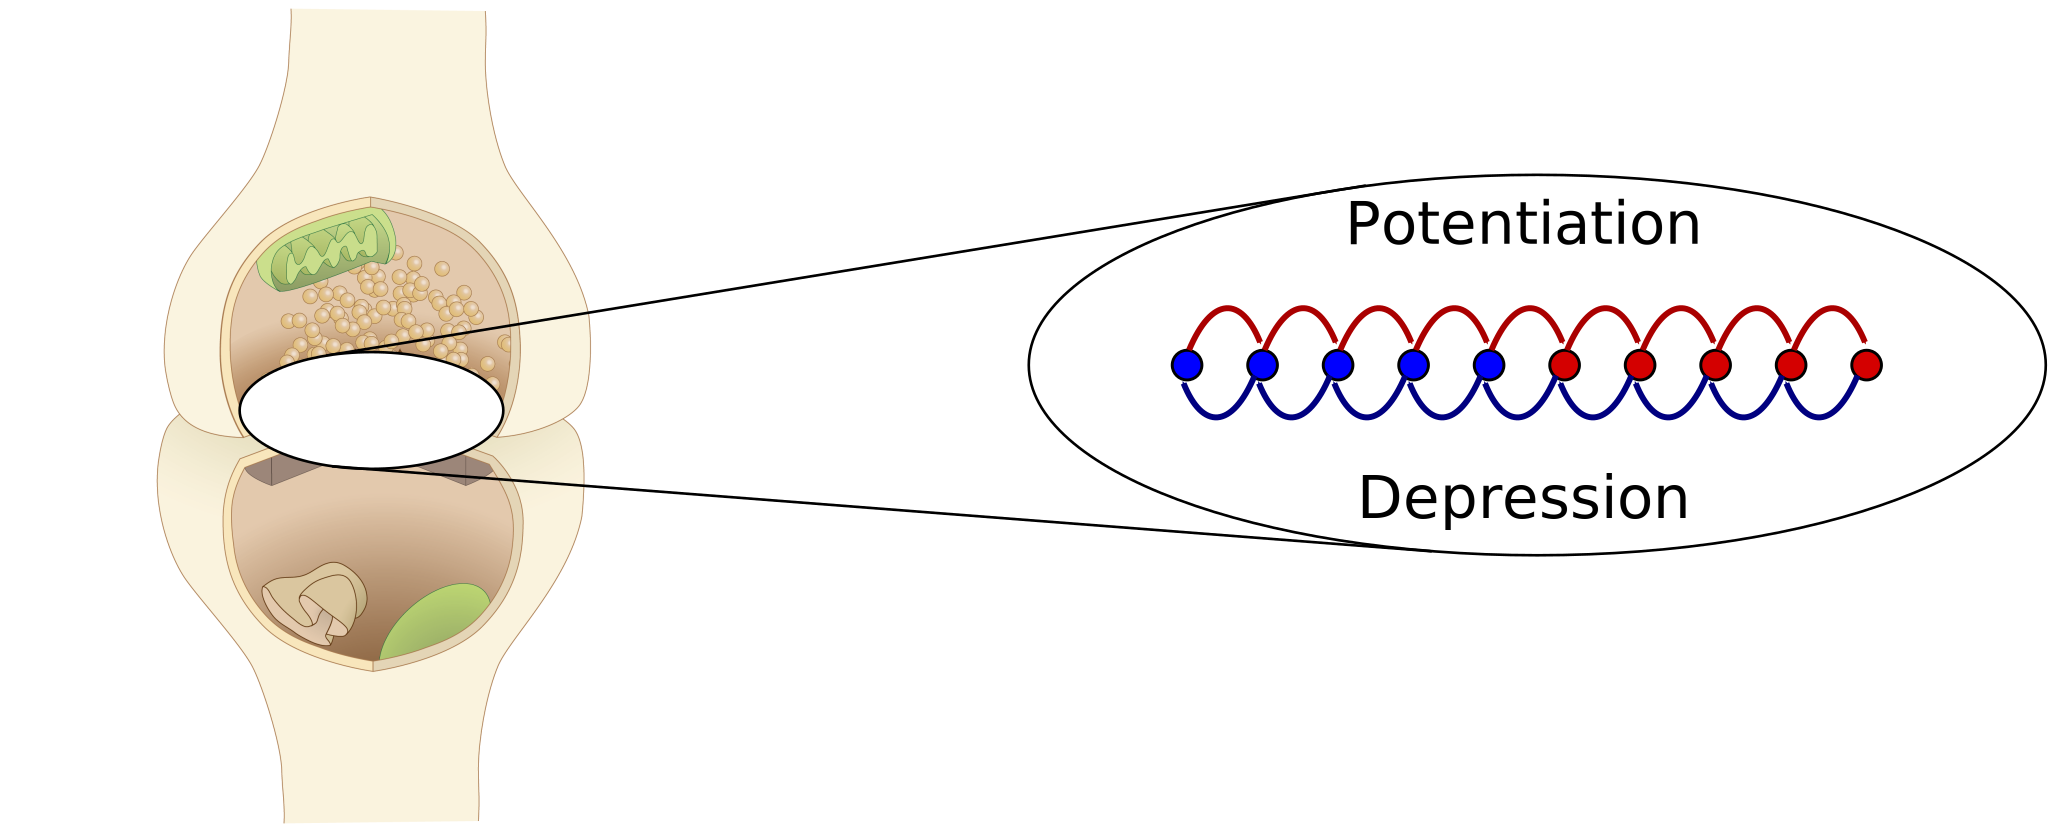
\includegraphics[width=0.7\linewidth]{serial_internal.svg}}}%
    \only<3->{\vp}
    \only<3>{\aligntop{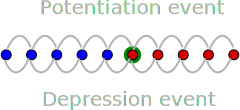
\includegraphics[width=0.5\linewidth]{Animation/serial_anim_01.svg}}}%
    \only<4>{\aligntop{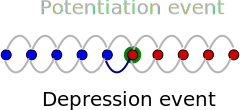
\includegraphics[width=0.5\linewidth]{Animation/serial_anim_02.svg}}}%
    \only<5>{\aligntop{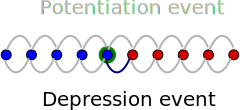
\includegraphics[width=0.5\linewidth]{Animation/serial_anim_03.svg}}}%
    \only<6>{\aligntop{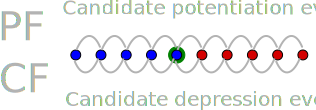
\includegraphics[width=0.5\linewidth]{Animation/serial_anim_04.svg}}}%
    \only<7>{\aligntop{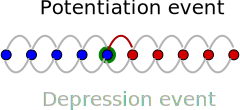
\includegraphics[width=0.5\linewidth]{Animation/serial_anim_05.svg}}}%
    \only<8>{\aligntop{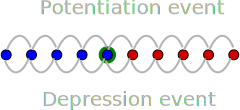
\includegraphics[width=0.5\linewidth]{Animation/serial_anim_06.svg}}}%
    \only<9>{\aligntop{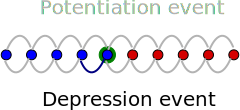
\includegraphics[width=0.5\linewidth]{Animation/serial_anim_07.svg}}}%
    \only<10>{\aligntop{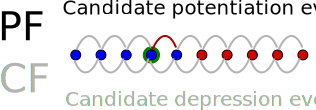
\includegraphics[width=0.5\linewidth]{Animation/serial_anim_08.svg}}}%
    \only<11>{\aligntop{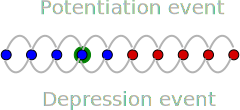
\includegraphics[width=0.5\linewidth]{Animation/serial_anim_09.svg}}}%
    \only<12>{\aligntop{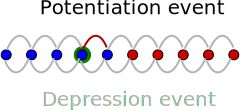
\includegraphics[width=0.5\linewidth]{Animation/serial_anim_10.svg}}}%
    \only<13>{\aligntop{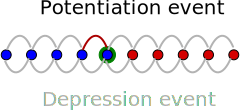
\includegraphics[width=0.5\linewidth]{Animation/serial_anim_11.svg}}}%
    \only<14>{\aligntop{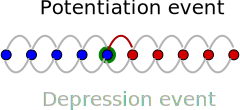
\includegraphics[width=0.5\linewidth]{Animation/serial_anim_12.svg}}}%
    \only<15>{\aligntop{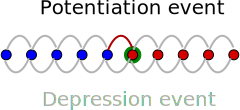
\includegraphics[width=0.5\linewidth]{Animation/serial_anim_13.svg}}}%
    \only<16>{\aligntop{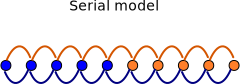
\includegraphics[width=0.5\linewidth]{Animation/serial.svg}}}%
%    \only<5>{\aligntop{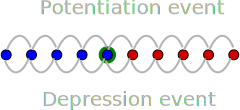
\includegraphics[width=0.5\linewidth]{Animation/serial_anim_06.svg}}}%
%    \only<6>{\aligntop{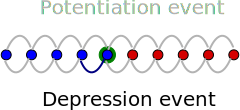
\includegraphics[width=0.5\linewidth]{Animation/serial_anim_07.svg}}}%
%    \only<7>{\aligntop{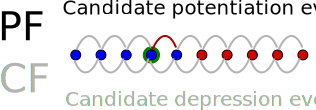
\includegraphics[width=0.5\linewidth]{Animation/serial_anim_08.svg}}}%
%    \only<8>{\aligntop{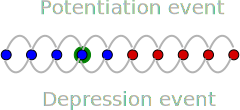
\includegraphics[width=0.5\linewidth]{Animation/serial_anim_09.svg}}}%
%    \only<9>{\aligntop{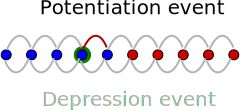
\includegraphics[width=0.5\linewidth]{Animation/serial_anim_10.svg}}}%
%    \only<10>{\aligntop{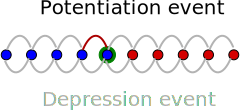
\includegraphics[width=0.5\linewidth]{Animation/serial_anim_11.svg}}}%
%    \only<11>{\aligntop{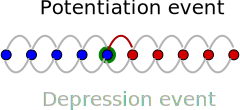
\includegraphics[width=0.5\linewidth]{Animation/serial_anim_12.svg}}}%
%    \only<12>{\aligntop{\includegraphics[width=0.5\linewidth]{Animation/serial_anim_13.svg}}}%
%    \only<13>{\aligntop{\includegraphics[width=0.5\linewidth]{Animation/serial.svg}}}%
    %
%    \hspace{0.05\linewidth}\parbox[t]{0.45\linewidth}{\raggedright
%    \visible<15>{
%    Mutation: transition probabilities \\ \vp
%    Training: rates of pot/dep events \\ \vp
%    Learning: synaptic weight}}
  \end{center}
\end{overlayarea}

%  \onslide<2>{\hfill
%  \parbox[t]{0.3\linewidth}{PF+\cancel{CF} \lto\ LTP, \\
%              PF+CF \lto\ LTD.}
%  \parbox[t]{0.27\linewidth}{Lower threshold\\ for LTD}
%  \parbox[t]{0.27\linewidth}{VOR gain increase}}
\vp
\begin{overlayarea}{0.95\linewidth}{0.3\textheight}
  \only<2>{States: \parbox[t]{0.85\linewidth}{\#AMPAR, \#NMDAR, NMDAR subunit composition, \\
   CaMK II autophosphorylation, activating PKC, p38 MAPK,...}

  \vp\footnotesize\citerr{Fusi2005cascade,Fusi2007multistate,Barrett2008discrete}}%
  %\\\citerr{Smith2006savings,Lahiri2013synapse}}%

  \only<9->{Metaplasticity: \parbox[t]{0.7\linewidth}{%
     change propensity for plasticity \\
     (independent of change in synaptic weight).}}
\end{overlayarea}

  %
  \note[item]{complex synapse: not just synaptic weight. dynamical system}
  \note[item]{important for memory with bounded synapses}
  \note[item]{nodes \lto\ states}
  \note[item]{color \lto\ sttrength}
  \note[item]{arrows \lto\ plasticity}
%  \note[item]{stoch process has steady state distribution.}
%  \note[item]{Prior activity puts it in this state. row vec.}
  \note[item]{plasticity events at rate r. indep at each synapse.}
  \note[item]{fraction pot/dep}
  \note[item]{Readout: synaptic weight vec when in each state.}
    \note[item]{Mutation: lower threshold \lto\ increase transition probs}
    \note[item]{Training: Changes statistics of LTP/LTD. Only parameters we have. Don't care about $r$.}
    \note[item]{Learning: Only output we have. Don't keep track of synaptic identity.}
%    \note<2>[item]{Same PF+CF input \lto\ same $r,f\pot,f\dep$ in each case.}
%    \note<2>[item]{Input to Pk, some linear combination of $\w$'s. }
% At $t=0$, the memory is created by $\M\potdep$ with probability $f\potdep$.
% \note[item]{for this one, we keep track of pot/dep, look for inc/dec of $\w$}
%
% \vp Forgetting caused by subsequent memories, evolving as
%
%  \begin{equation*}
%  \begin{aligned}
%    \diff{\pr(t)}{t} &= r\pr(t)\frg,
%    &\qquad
%    \frg &= f\pot\M\pot+f\dep\M\dep-\I,\\&&
%    \eq\frg &=0.
%  \end{aligned}
%  \end{equation*}
%%
%  \note[item]{Memory at $t=0$, keep track of pot/dep}
%  \note[item]{subsequent: average over pot/dep}
% \note[item]{$\frg$ is forgetting matrix, $\I=$identity, don't keep track of pot/dep}
% Eventually, this will settle into the equilibrium distribution:
% %
% %
% \note[item]{In equilibrium prior to memory creation}
%
\end{frame}

%-------------Slide--------------------------------------------------------

\begin{frame}{Example models}
%
 Two example models of complex synapses.
 %
 \begin{center}
  \aligntop{\includegraphics[width=4cm]{cascade.svg}}
  \hspace{2cm}
  \aligntop{\includegraphics[width=4cm]{multistate.svg}}
 \end{center}
 \citerr{Fusi2005cascade,Leibold2008serial,Ben-DayanRubin2007sparse}
 %
 \note[item]{previous work, also: Benna-Fusi}

 These have different memory storage properties
 %
 \begin{center}
 \includegraphics[width=0.5\linewidth]{cascms.svg}
 \end{center}
 %
 \note[item]{Multistate good at one time, bad at others,}
 \note[item]{Cascade, less well at that time, better over range of times.}
%
\end{frame}

%-------------Slide--------------------------------------------------------

\begin{frame}[label=fr_questions]{Questions}
%
 \begin{itemize}
   \item Can we understand the space of \emph{all possible} synaptic models?
   \note[item]{not just individual models}
   \item How does structure \hyperlink{fr_net<1>}{(topology)} of model $\to$ function (memory curve)?
   \note[item]{understand net (link on topology)}
   \item What are the limits on what can be achieved?
   \note[item]{avoid using word ``optimal''. depends on what want to do.}
   \item Which transition topologies saturate these limits?
   \item Can synaptic structure be tuned for different timescales of memory?
 \end{itemize}
%
\end{frame}

%%-------------Slide--------------------------------------------------------
%
%\begin{frame}{Simplifying assumptions}
%%
%\begin{itemize}
%  \item No spatial/temporal correlations in plasticity events.
%      %
%      \note[item]{allows us to concentrate on synapse, not neuron/network}
%      %
%%  \item Which synapses eligible for plasticity chosen randomly.
%      %
%      \note[item]{No filing system}
%      %
%  \item Candidate plasticity events $\sim$ Poisson processes.% with rates $rf\potdep$, where $f\pot+f\dep=1$.
%      %
%      \note[item]{don't care if STDP...}
%%      %
%%      \note[item]{$r=$ total rate of plasticity events per synapse, $f\potdep=$ fraction of events that are potentiating/depressing.}
%      %
%  \item Potentiation and depression $\sim$ Markov processes.% with transition probabilities $\M\potdep$.
%%      %
%%      \note[item]{matrix elements: transition prob from $i\to j$, given pot/dep}
%  \item Ideal observer: read weights directly.
%      \note[item]{not electrical activity: don't model neurons/network}
%      \note[item]{upper bound on electrical activity readout}
%      %
%  \item Synaptic weights can only take 2 values.
%      %
%  \citerr{Fusi2005cascade,Fusi2007multistate,Barrett2008discrete}
%      %
%      \note[item]{looks like binary synapse from outside. Inside...}
%\end{itemize}
%%
%\end{frame}
%
%-------------Slide--------------------------------------------------------

\begin{frame}{Parameters for synaptic dynamics}
%
  There are $N$ identical synapses with $M$ internal functional states.
  %
  \begin{center}
    \includegraphics[width=0.7\linewidth]{model.svg}
  \end{center}
  %
  \note[item]{stoch process has steady state.}
  \note[item]{Prior activity puts it in this state. row vec.}
  \note[item]{plasticity events at rate r}
  \note[item]{fraction pot/dep}
  \note[item]{probs changed by Markov matrices, prob $i\to j$}
  \note[item]{Readout: synaptic weight vec when in each state.}
  \vp
% At $t=0$, the memory is created by $\M\potdep$ with probability $f\potdep$.
% \note[item]{for this one, we keep track of pot/dep, look for inc/dec of $\w$}
%
% \vp Forgetting caused by subsequent memories, evolving as
%
  \begin{equation*}
  \begin{aligned}
    \diff{\pr(t)}{t} &= r\pr(t)\frg,
    &\qquad
    \frg &= f\pot\M\pot+f\dep\M\dep-\I,\\&&
    \eq\frg &=0.
  \end{aligned}
  \end{equation*}
%
  \note[item]{Memory at $t=0$, keep track of pot/dep}
  \note[item]{subsequent: average over pot/dep}
% \note[item]{$\frg$ is forgetting matrix, $\I=$identity, don't keep track of pot/dep}
% Eventually, this will settle into the equilibrium distribution:
% %
% %
% \note[item]{In equilibrium prior to memory creation}
%
\end{frame}

%%-------------Slide--------------------------------------------------------
%
%\begin{frame}{Memory curve}
%%
% $\syn$ is the $N$-element vector of synaptic weights.
% %
% \note[item]{of different synapses}
% \note[item]{ideal observer reads weights, not states}
% \note[item]{upper bound on electrical activity readout}
% %
% \begin{equation*}
%   \begin{aligned}
%     \text{Signal} &= \av{\synid \cdot \syn(t) -  \synid \cdot \syn(\infty)},\\
%     \text{Noise} &= \sqrt{\var\prn{\synid \cdot \syn(\infty)}} \sim \sqrt{N}.
%   \end{aligned}
% \end{equation*}
% %
% \note[item]{ideal: pot$\to$strong...}
% \note[item]{use $\synid \cdot \syn(\infty)$ as null model}
% \note[item]{Noise: ignore correction when asymmetric. No effect.}
%% \note[item]{if we ignore correlations...}
%% %
%% Related to reconstruction probability of single synapses.
%% %
%% \begin{equation*}
%%   \SNR(t) \sim \sqrt{N}\,P(\text{strong/weak},t|\text{pot/dep},t=0)-\ldots(t=\infty).
%% \end{equation*}
%% %
%  We find:
% %
% \begin{equation*}
%   \snr(t) =
%%      \frac{\sqrt{N}(2f\pot f\dep)}{\sqrt{4\eq_+\eq_-}}\,
%      \sqrt{N}(2f\pot f\dep)\,
%      \eq \prn{\M\pot-\M\dep} \exp\prn{rt\frg}\w.
% \end{equation*}
% %
% \note[item]{Using $\frg$ averages over pot/dep sequence (proof: expand)}
%%
%\end{frame}
%
%-------------Slide--------------------------------------------------------

\begin{frame}{Constraints}
%
 Memory curve given by
 %
 \begin{equation*}
 \begin{aligned}
   \snr(t) &=
%      \frac{\sqrt{N}(2f\pot f\dep)}{\sqrt{4\eq_+\eq_-}}\,
      \sqrt{N}(2f\pot f\dep)\,
      \eq \prn{\M\pot-\M\dep}      \exp\prn{rt\frg} \w, \\
   \snrb(\tau) &=
      \sqrt{N}(2f\pot f\dep)\,
      \eq \prn{\M\pot-\M\dep}      \brk{\I - r\tau\frg}\inv \w. \\
 \end{aligned}
 \end{equation*}
 %
 \note[item]{prefactors don't do anything, ignore}
 \note[item]{prior state, encoding, forgetting, readout}
 %
 Constraints: \qquad $\M\potdep_{ij}\in[0,1]$, \qquad $\sum_j\M\potdep_{ij}=1$.
 %
 \note[item]{difficult to to apply}

 \vp Eigenmode decomposition:
 %
 \begin{equation*}
 \begin{aligned}
   \snr(t) &= \sqrt{N}\sum_a \initial_a \,\e^{-rt/\tau_a}, \\
   \snrb(\tau) &= \sqrt{N}\sum_a \frac{\initial_a }{1+r\tau/\tau_a}, \\
 \end{aligned}
 \end{equation*}
 %
 \note[item]{what are constraints on these?}
%
\end{frame}


%-------------Section--------------------------------------------------------

\section{Upper bounds}


%-------------Slide--------------------------------------------------------

\begin{frame}{Upper bounds on measures of memory}
%
 Initial SNR:
 %
 \begin{equation*}
   \snr(0) = \snrb(0) \leq \sqrt{N}.
 \end{equation*}
 %
 %
 \begin{center}
   \includegraphics[height=0.1\linewidth]{binary_det.svg}
 \end{center}
 %
 Area under curve:
 %
 \begin{equation*}
   \area = \intd[_0^\infty]{t} \snr(t) = \lim_{\tau\ra\infty} \tau \, \snrb(\tau) \leq \sqrt{N}(M-1)/r.
 \end{equation*}
 %
 %
 \begin{center}
   \includegraphics[height=0.1\linewidth]{multistate_sticky.svg}
 \end{center}
 %
 \citerr{Lahiri2013synapse}
%
\end{frame}

%-------------Section--------------------------------------------------------

\subsection{Initial SNR}

%-------------Slide--------------------------------------------------------

\begin{frame}{Initial SNR as flux}
%
 Initial SNR is closely related to flux between strong \& weak states
 %
 \note[item]{flux = eq prob $\times$ trans prob}
 %
 \begin{equation*}
   \SNR(0) \leq \frac{4\sqrt{N}}{r}\,\F_{-+}.
 \end{equation*}
 %
 \note[item]{usually saturated: pot never dec, dep never inc}
 Max when {\parbox[t]{8cm}{potentiation guarantees $\w\to+1$,\\
 depression guarantees $\w\to-1$.}}
 %
 \begin{center}
   \includegraphics[height=3cm]{max_init_pot.svg}
   \hp \hp
   \includegraphics[height=3cm]{max_init_dep.svg}
 \end{center}
 %
 \note[item]{transitions out of one node sum to 1}
 \note[item]{equivalent to two-state model: doesn't matter which strong/weak state, same prob of going to other set.}
%
\end{frame}

%-------------Slide--------------------------------------------------------

\begin{frame}{Two-state model}
%
 Two-state model equivalent to previous slide:
  \begin{center}
  Transitions:
   \parbox{2cm}{\includegraphics[height=2cm]{binary_det.svg}}
   $\implies\snr(t)=\sqrt{N}\,(4 f\pot f\dep)\,\e^{-rt}.$
  \end{center}
  \note[item]{decays very quickly}

 \vp Maximal initial SNR:\note[item]{$f\pot=\half$}
 %
 \begin{equation*}
   \snr(0) \leq \sqrt{N}.
 \end{equation*}
 %
 \note[item]{Initial SNR not a good thing to optimise.}
%
\end{frame}

%-------------Section--------------------------------------------------------

\subsection{Area under memory curve}

%-------------Slide--------------------------------------------------------

\begin{frame}{Area under memory curve}
%
  %
  \begin{equation*}
    \area = \intd[_0^\infty]{t} \snr(t),
    \qquad
    \snrb(\tau) \ra \frac{\area}{\tau}
    \quad \text{as} \quad \tau \ra \infty.
  \end{equation*}
%


  \vp\parbox{5cm}{
  Area bounds memory lifetime:\\
  %
  \begin{equation*}
  \begin{aligned}
    \SNR(\text{lifetime})&=1
    \\
    \implies
    \quad
    \text{lifetime} &< \area.
  \end{aligned}
  \end{equation*}
  %
  }
  \parbox{6.5cm}{
    \includegraphics[width=6cm]{lifetime.eps}
  }
  %
  \note[item]{lifetime = area under green < area under blue}
  \note[item]{capacity $\sim r$ lifetime, \#new memories before we forget original.}

  %
  \vp This area has an upper bound:
  %
  \begin{equation*}
    \area \leq \sqrt{N}(M-1)/r.
  \end{equation*}
  %
  \note[item]{reminder: $N=$\#synapses, $M=$\#states}
  Saturated by a model with linear chain topology.
  \note[item]{proof next slide}
%
\end{frame}

%-------------Slide--------------------------------------------------------

\begin{frame}[label=fr_areaproof]{Proof of area bound}
%
 For any model, we can construct perturbations that
 \parbox[c]{5cm}{
  \begin{itemize}
    \item preserve equilibrium distribution,
    \item increase area.
  \end{itemize}
  \hyperlink{fr_tech}{\beamerbutton{details}}
  %
  \note[item]{relies on order \& technical condition}
 }
 \parbox[c]{5cm}{
  %
  \begin{center}
    \includegraphics[width=4cm]{shortcut.svg}
  \end{center}
  %
 }\\
 \eg decrease ``shortcut'' transitions, increase bypassed ``direct'' ones.\\
 Endpoint: linear chain

 \vp The area of this model is
 %
 \begin{equation*}
   A = \frac{2\sqrt{N}}{r}\sum_k \eq_k \abs{k-\av{k}}.
 \end{equation*}
 %
 \note[item]{max given $\eq$}
 \note[item]{now max \wrt $\eq$}
 Max: equilibrium probability distribution concentrated at both ends.
 \note[item]{keep c.o.m.\ in middle}
 \\
 \citerr{Barrett2008discrete}
 \note[item]{similar result, slightly different conditions: linear weights, mutual info}
%
\end{frame}

%-------------Slide--------------------------------------------------------

\begin{frame}{Saturating model}
%
 Make end states ``sticky''
 %
 \begin{center}
   \includegraphics[width=8cm]{multistate_sticky.svg}
 \end{center}
 %
 Has long decay time, but terrible initial SNR.
 %
 \note[item]{Difficult to get out of end state.}
 \note[item]{Area not a good thing to optimise}
 %
 \begin{equation*}
   \lim_{\varepsilon\to0}A=\sqrt{N}(M-1)/r.
 \end{equation*}
 %
%
\end{frame}


%-------------Section--------------------------------------------------------

\section{Envelope memory curve}

%-------------Slide--------------------------------------------------------

\begin{frame}{Bounding finite time SNR}
%
 SNR curve:
 %
 \begin{equation*}
  \begin{aligned}
%   \snr(t) &= \sqrt{N}\sum_a \initial_a \,\e^{-rt/\tau_a}, \\
   \snrb(\tau) &= \sqrt{N}\sum_a \frac{\initial_a }{1+r\tau/\tau_a}, \\
 \end{aligned}
 \end{equation*}
 %
 \note[item]{from eigenmode decomposition}
 subject to constraints:
 %
 \begin{equation*}
   \sum_a \initial_a \leq 1,
   \qquad
   \sum_a \initial_a\, \tau_a \leq M-1.
 \end{equation*}
 %
 \note[item]{from initial, area bounds}
 We can maximise \wrt $\initial_a,\tau_a$.
%
\end{frame}

%%-------------Slide--------------------------------------------------------
%
%\begin{frame}{Constructing the envelope}
%%
% %
% \begin{center}
% \begin{overlayarea}{10cm}{4.5cm}
%   \only<1>{\includegraphics[width=8cm]{env2_t1.eps}}
%   \only<2>{\includegraphics[width=8cm]{env2_t2.eps}}
%   \only<3>{\includegraphics[width=8cm]{env2_all.eps}}
%%   \only<4>{\includegraphics[width=8cm]{env2_ex.eps}}
% \end{overlayarea}
% \end{center}
% %
% \begin{overlayarea}{10cm}{3cm}
%  \only<1>{Maximise SNR at one time}
%  %
%  \note<1->[item]{One exp. only constrains SNR at that time, not others}
%  %
%  \only<2>{Another time}
%  %
%  \note<2->[item]{get another bound}
%  %
%  \only<3>{All times $\to$ envelope}
%  %
%  \note<3->[item]{vary time of max. no curve can cross this.}
%  \note<3->[item]{Regions: init(1); area(1,2)}
%  \note<3->[item]{Early: exp; Late: power-law, $\sim t\inv$}
%  \note<3->[item]{snr(lifetime)=1. Bounded by envelope=1.}
%  \note<3->[item]{is it tight? can any constrained set of exps be acheived?}
% %
% \only<3>{
% \begin{equation*}
% \begin{aligned}
%%   N &> \CO(M^2) &\implies
%   \text{lifetime} &\leq \frac{\sqrt{N}(M-1)}{\e r}, \\
%%   N &< \CO(M^2) &\implies
%%   \text{lifetime} &\leq \frac{\gamma^2{N}}{2\e r}.
% \end{aligned}
% \end{equation*}
% }
% %
%  %
%%  \only<4>{Memory curves of example models.}
%%  %
%%  \note<4->[item]{no}
%%  \note<4->[item]{One exp. discuss models next slide}
% \end{overlayarea}
%%
%\end{frame}
%
%

%-------------Slide--------------------------------------------------------

\begin{frame}{Proven envelope: memory frontier}
%
 Upper bound on memory curve at \emph{any} time.

\vp
\parbox[c]{0.55\linewidth}{
 \begin{center}
   \aligntop{\includegraphics[width=0.9\linewidth]{LenvProven.svg}}
 \end{center}
}
\hspace{0.02\linewidth}
\parbox[c]{0.4\linewidth}{
 %
   Initial SNR: %deterministic binary synapse
   %
   \begin{center}
  %   \includegraphics[width=6cm]{multistate_shorten.svg}
     \includegraphics[height=0.15\linewidth]{binary_det.svg}
   \end{center}
   %
  % \note[item]{shorten length of chain, keeping deterministic}

   %
   \vp Late times: %serial model with ``sticky'' end states
   %
   \begin{center}
     \includegraphics[height=0.15\linewidth]{multistate_sticky.svg}
   \end{center}
   %
}

 \citerr{Lahiri2013synapse}

 \vp No model can ever go above this envelope.
 Is it achievable?
%
\end{frame}

%-------------Slide--------------------------------------------------------

\begin{frame}{Achievable envelope}
%
 %
% \begin{center}
 \parbox[c]{0.67\linewidth}{
   \aligntop{\includegraphics[width=0.95\linewidth]{LenvNum.svg}}
   \note[item]{Best we've found, by numerical opt and hand chosen models.}
% \note[item]{Models on next slide}
 }
% \end{center}
% \hspace{0.01\linewidth}
 %
 \parbox[c]{0.3\linewidth}{
   Serial topology:
   %
   \begin{center}
  %   \includegraphics[width=6cm]{multistate_shorten.svg}
     \includegraphics[width=0.99\linewidth]{multistate_uni.svg}
   \end{center}
   %
 }
 \note[item]{Gap $\sim\CO(\sqrt{N})$.}
 \note[item]{Area bound active at early times $\implies$ need more constraints.}
%
\end{frame}


%-------------Slide--------------------------------------------------------

\begin{frame}{Models that maximise memory for one timescale}
%
 %
 \begin{center}
   \only<1>{\aligntop{\includegraphics[width=0.9\linewidth]{Animation/Lenv27.svg}}}%
   \only<2>{\aligntop{\includegraphics[width=0.9\linewidth]{Animation/Lenv30.svg}}}%
   \only<3>{\aligntop{\includegraphics[width=0.9\linewidth]{Animation/Lenv34.svg}}}%
   \only<4>{\aligntop{\includegraphics[width=0.9\linewidth]{Animation/Lenv42.svg}}}%
   \only<5>{\aligntop{\includegraphics[width=0.9\linewidth]{Animation/Lenv47.svg}}}%
   \only<6>{\aligntop{\includegraphics[width=0.9\linewidth]{Animation/Lenv51.svg}}}%
   \only<7>{\aligntop{\includegraphics[width=0.9\linewidth]{Animation/Lenv27.svg}}}%
   \only<8>{\aligntop{\includegraphics[width=0.9\linewidth]{Animation/Lenv24.svg}}}%
   \only<9>{\aligntop{\includegraphics[width=0.9\linewidth]{Animation/Lenv21.svg}}}%
   \only<10>{\aligntop{\includegraphics[width=0.9\linewidth]{Animation/Lenv20.svg}}}%
   \only<11>{\aligntop{\includegraphics[width=0.9\linewidth]{Animation/Lenv19.svg}}}%
   \only<12>{\aligntop{\includegraphics[width=0.9\linewidth]{Animation/Lenv17.svg}}}%
   \only<13>{\aligntop{\includegraphics[width=0.9\linewidth]{Animation/Lenv16.svg}}}%
   \only<14>{\aligntop{\includegraphics[width=0.9\linewidth]{Animation/Lenv14.svg}}}%
   \only<15>{\aligntop{\includegraphics[width=0.9\linewidth]{Animation/Lenv12.svg}}}%
   \only<16>{\aligntop{\includegraphics[width=0.9\linewidth]{Animation/Lenv06.svg}}}%
   \only<17>{\aligntop{\includegraphics[width=0.9\linewidth]{Animation/Lenv01.svg}}}%
 \end{center}
%
%
\end{frame}


%-------------Slide--------------------------------------------------------

\begin{frame}{Heuristic envelope}
%
 %
 \begin{center}
   \includegraphics[width=0.88\linewidth]{LenvHeuristic.svg}
 \end{center}
%
%
\end{frame}

%-------------Slide--------------------------------------------------------

\begin{frame}{Synaptic structures for different timescales of memory}
%
 Real synapses limited by molecular building blocks. \\
 Evolution had larger set of priorities.

 \vp What can we conclude?

 \begin{center}
 \begin{tabular}{ccccc}
   % after \\: \hline or \cline{col1-col2} \cline{col3-col4} ...
   Short timescales & $\longrightarrow$ & Intermediate timescales & $\longrightarrow$ & Long timescales \\[0.5cm]
   \alignmid{\includegraphics[height=0.05\linewidth]{binary_det.svg}} & $\longrightarrow$ & \alignmid{\includegraphics[height=0.05\linewidth]{multistate_uni.svg}} & $\longrightarrow$ & \alignmid{\includegraphics[height=0.05\linewidth]{multistate_sticky.svg}} \\[0.5cm]
   \visible<2->{short \& wide} & \visible<2->{$\longrightarrow$} & \visible<2->{long \& thin} &  &  \\[0.5cm]
    & & \visible<3->{strong transitions} & \visible<3->{$\longrightarrow$} & \visible<3->{weak transitions} \\
 \end{tabular}
 \end{center}
%
\end{frame}

%%-------------Slide--------------------------------------------------------
%
%\begin{frame}{Best models at single times}
%%
% Early times:
% %
% \begin{center}
%%   \includegraphics[width=6cm]{multistate_shorten.svg}
%   \includegraphics[width=6cm]{diffjump.svg}
% \end{center}
% %
%% \note[item]{shorten length of chain, keeping deterministic}
% \note[item]{vary length, keeping deterministic}
% %
% Late times:
% %
% \begin{center}
%   \includegraphics[width=6cm]{multistate_sticky.svg}
% \end{center}
% %
% \note[item]{Area maximising.}
%% \note[item]{two mechs for slowing forgetting: time (lower trans prob) and space (diffusion length)}
% %
%%
%\end{frame}
%
%%-------------Slide--------------------------------------------------------
%
%\begin{frame}{Additional constraint}
%%
% Conjecture: additional constraint
% %
% \begin{equation*}
%   \initial_a\sqrt{\tau_a} \leq \CO(1).
% \end{equation*}
% %
% \note[item]{Tested experimentally. Discuss later}
% %
% Saturated by a diffusive chain:
% %
% \begin{equation*}
%   \SNR(0) \sim \frac{1}{M},
%   \qquad
%   \text{time-scale} \sim M^2.
% \end{equation*}
% %
%%
%\end{frame}
%
%%-------------Slide--------------------------------------------------------
%
%\begin{frame}{Envelope 2}
%%
% %
% \begin{center}
%   \includegraphics[width=8cm]{env23.eps}
% \end{center}
% %
% \note[item]{dashed: conjecture. tight.}
%
% %
% \begin{equation*}
% \begin{aligned}
%   rt &< \CO(M^2), &\quad
%   \text{envelope} &\sim (rt)^{-1/2}, \\
%   rt &> \CO(M^2), &
%   \text{envelope} &\sim (rt)^{-1} .
% \end{aligned}
% \end{equation*}
% %
% \note[item]{earlier: diffusion limited. later: stochastic limited.}
% \note[item]{regions: init(1); sqrt(2,3); area(3,4)}
% \note[item]{Benna-Fusi hugs envelope? cascade $\sim t^{-3/4}$}
%%
%\end{frame}
%
%%-------------Slide--------------------------------------------------------
%
%\begin{frame}{Lifetime bound}
%%
% Lifetime of a memory bounded by where envelope crosses 1
% %
% \begin{equation*}
% \begin{aligned}
%%   N &> \CO(M^2) &\implies
%   \text{lifetime} &\leq \frac{\sqrt{N}(M-1)}{\e r}, \\
%%   N &< \CO(M^2) &\implies
%%   \text{lifetime} &\leq \frac{\gamma^2{N}}{2\e r}.
% \end{aligned}
% \end{equation*}
% %
%% \note[item]{$\gamma\sim\CO(1)$ constant in additional constaint}
%% \note[item]{First $t^{-1}$ assumes M low. Second $t^{-1/2}$ applies to Benna-Fusi.}
% \note[item]{Independent synapses?}
%%
%\end{frame}
%
%%-------------Slide--------------------------------------------------------
%
%\begin{frame}{Additional constraint: other forms?}
%%
% Involving eigenmodes:
% %
% \begin{equation*}
%   \initial_a \sqrt{\tau_a},
%   \qquad
%   \sum_a \initial_a \sqrt{\tau_a},
%   \qquad
%   \sum_a \initial_a^2 {\tau_a}.
% \end{equation*}
% %
% \note[item]{as one-time max only involved one exp, would also work}
% \note[item]{right units}
% %
% Not involving eigenmodes
% %
% \begin{equation*}
%   \area \times \snr(0),
%   \qquad
%   \intd{t} \snr(t)^2.
% \end{equation*}
% %
% \note[item]{easier to work with?}
% \note[item]{L2 doesn't have nice expression in terms of matrices}
%%
%\end{frame}
%
%%-------------Slide--------------------------------------------------------
%
%\begin{frame}{Cheeger inequality}
%%
% \parbox{5cm}{
% Cheeger constant:
% %
% \begin{equation*}
%   \phi \equiv \min_\CS \brc{\frac{\operatorname{Perimeter}(\p\CS)}{\operatorname{Area}(\CS)}}.
% \end{equation*}
% %
% \note[item]{split into two pieces. pick smaller. higher dim.}
% \note[item]{bottleneck}
% }
% \parbox{6cm}{
%   \includegraphics[width=5cm]{dumbbell.svg}
% }
% Timescale for diffusion to equilibriate
% %
% \begin{equation*}
%   \frac{1}{D \tau_{\text{diffusion}}} > \CO(1)\, \phi^2.
% \end{equation*}
% %
% \note[item]{if we want slow diffusion, need lhs small $\to$ need bottleneck.}
% \note[item]{purely geometric}
% \note[item]{also inequality in other direction: want slow diffusion $\to$ need bottleneck. Not useful for us}
%%
%\end{frame}
%
%%-------------Slide--------------------------------------------------------
%
%\begin{frame}{Cheeger inequality: Markov chains}
%%
% Cheeger constant:
% %
% \begin{equation*}
%   \phi \equiv \min_\CS \brc{\frac{\F_{\CS\CS\comp}}{\eq(\CS)}}.
% \end{equation*}
% %
% \note[item]{split states into two subsets. pick smaller.}
% \note[item]{again bottleneck}
% \note[item]{denominator varies}
% %
% Timescale to equilibriate:
% %
% \begin{equation*}
%   \frac{1}{\max_a\tau_a} > \CO(1)\, \phi^2.
% \end{equation*}
% %
% Simple proof assuming detailed balance. \citerr{Sinclair1989cheeger}\\
% More complicated proof for general case. \citerr{Lawler1988cheeger}
% %
% \note[item]{$\CO(1)$ bit differs}
% \note[item]{bottleneck need not be between strong \& weak.}
%%
%\end{frame}
%
%%-------------Slide--------------------------------------------------------
%
%\begin{frame}{Counter examples?}
%%
% Put bottleneck somewhere else:
% %
% \begin{center}
%   \includegraphics[width=6cm]{multistate_counter.svg}
% \end{center}
% %
% \note[item]{eq prob concentrated near middle. bottleneck at $\epsilon$.}
% %
% Set $\epsilon = 1/M$, see how putative constraints vary:
% %
% \begin{center}
%   \includegraphics[width=6cm]{counter_graph.eps}
% \end{center}
% %
% \note[item]{high inital snr and long timescale in different modes.}
% \note[item]{only eigenmode dependent constraints survive (and L2 - but difficult to work with).}
%
% Also tried: random Markov chains.
%%
%\end{frame}
%
%%-------------Slide--------------------------------------------------------
%
%\begin{frame}{Two-time envelope}
%%
% Maximise $\snr(t_1)$ subject to constraint $\snr(t_2)=S_2$.
% %
%
% \vp For $t_1$ close to $t_2$, get single exponential.\\
%  Far away, get two exponentials.
% %
% \note[item]{Max at multiple times, $\to$ multiple timescales? cascade? Benna-Fusi?}
%
% \vp See tradeoff between $\snr(t_1)$ and $\snr(t_2)$.
% %
%
% %
% \begin{center}
%   \includegraphics[width=5cm]{two_time_env.eps}
% \end{center}
% %
%\note[item]{only implemented first 2 constraints}
%  \note[item]{numerics not working. 2 exp solution need to solve 2 transcendental equations.}
%%
%\end{frame}
%

%-------------Section--------------------------------------------------------

\section{Experimental tests?}

%-------------Slide--------------------------------------------------------

\begin{frame}{Proposed Experimental design}
%
 Subject a synapse to a sequence of candidate plasticity events.

 Observe the changes in synaptic efficacy.

 \begin{center}
     \only<1>{\aligntop{\includegraphics[width=0.1\linewidth]{single_synapse_depstrong.svg}}}%
     \only<2>{\aligntop{\includegraphics[width=0.1\linewidth]{single_synapse_depweak.svg}}}%
     \only<3>{\aligntop{\includegraphics[width=0.1\linewidth]{single_synapse_potweak.svg}}}%
     \only<4>{\aligntop{\includegraphics[width=0.1\linewidth]{single_synapse_depweak.svg}}}%
     \only<5>{\aligntop{\includegraphics[width=0.1\linewidth]{single_synapse_potstrong.svg}}}%
     \only<6->{\aligntop{\includegraphics[width=0.1\linewidth]{single_synapse_potstrong.svg}}}%
 \end{center}

 \visible<7->{\textbf{EM algorithms:}

   Sequence of hidden states $\ra$ estimate transition probabilities \\
   Transition probabilities $\ra$ estimate sequence of hidden states

   \citerr{Baum1970baumwelch,rabiner1993speechrec,Dempster2007EM}

 \vp \textbf{Spectral algorithms:}

 Compute $P(w_1), P(w_1,w_2), P(w_1,w_2,w_3),\ldots$  \hp
 \parbox[t]{0.3\linewidth}{
   from data, \\
   from model.
 }

 \citerr{Hsu2008hmmspec}
 }
%
\end{frame}

%-------------Slide--------------------------------------------------------

\begin{frame}{Fitting algorithm}
%
 %
 \begin{center}
   \only<1>{\aligntop{\includegraphics[width=0.97\linewidth]{Animation/FitVid00.svg}}}%
   \only<2>{\aligntop{\includegraphics[width=0.97\linewidth]{Animation/FitVid104.svg}}}%
   \only<3>{\aligntop{\includegraphics[width=0.97\linewidth]{Animation/FitVid208.svg}}}%
   \only<4>{\aligntop{\includegraphics[width=0.97\linewidth]{Animation/FitVid312.svg}}}%
   \only<5>{\aligntop{\includegraphics[width=0.97\linewidth]{Animation/FitVid416.svg}}}%
   \only<6>{\aligntop{\includegraphics[width=0.97\linewidth]{Animation/FitVid520.svg}}}%
   \only<7>{\aligntop{\includegraphics[width=0.97\linewidth]{Animation/FitVid624.svg}}}%
   \only<8>{\aligntop{\includegraphics[width=0.97\linewidth]{Animation/FitVid728.svg}}}%
   \only<9>{\aligntop{\includegraphics[width=0.97\linewidth]{Animation/FitVid832.svg}}}%
   \only<10>{\aligntop{\includegraphics[width=0.97\linewidth]{Animation/FitVid939.svg}}}%
 \end{center}
 %
%
\end{frame}


%-------------Slide--------------------------------------------------------

\begin{frame}{Experimental problems}
%
 \begin{itemize}
   \item Need single synapses.
   \item Need long sequences of plasticity events.
   \item Need to control types of candidate plasticity events.
   \item Need to measure synaptic efficacies.
 \end{itemize}

 \vp When we patch the postsynaptic neuron \lto\ Ca washout.
%
\end{frame}

%-------------Slide--------------------------------------------------------

\begin{frame}{Summary}
%
  \begin{itemize}
    \item We have formulated a general theory of learning and memory with complex synapses.
%    \item We can impose an order on the internal states of a synapse through the theory of first passage times.
    \item The area under the memory curve of any model $<$ linear chain with same equilibrium distribution.
    \item We find a memory envelope: a single curve that cannot be exceeded by the memory curve of \emph{any} synaptic model.
    \item Synaptic complexity ($M$ internal states) raises the memory envelope linearly in $M$ for times $> \CO(M)$.
    \item We understood which types of synaptic structure are useful for storing memories for different timescales.
    \item Gap between envelope and what we can achieve at early times?
    \item Trade-off between SNR at different times?
%    \item For times $< \CO(M^2)$: conjecture that the model that reaches the envelope uses deterministic transitions $\to$ diffusive forgetting.
  \end{itemize}

%
\end{frame}





%-------------Slide--------------------------------------------------------
%
%% Press Ctrl-D to insert a new slide
%
%
%-------------Slide--------------------------------------------------------

\begin{frame}{Acknowledgements}
%
 Thanks to:
 \begin{itemize}
   \item Surya Ganguli
   \item Stefano Fusi
   \item Marcus Benna
   \item David Sussillo
   \item Jascha Sohl-Dickstein
 \end{itemize}
 \note[item]{Last slide!}
%
\end{frame}

%-------------Slide--------------------------------------------------------
\appendix
%-------------Slide--------------------------------------------------------

\begin{frame}[allowframebreaks]{References}
%

 {\small
 \bibliographystyle{unsrt_slides}
 \bibliography{maths,neuro,markov}
 }
%
\end{frame}

%-------------Slide--------------------------------------------------------

\begin{frame}[label=fr_tech]{Techinical detail: ordering states}
%
 Let $\fpt_{ij}=$ mean first passage time from state $i$ to state $j$.
 Then:
 %
 \begin{equation*}
   \eta = \sum_j \fpt_{ij} \eq_j,
 \end{equation*}
 %
 is independent of the initial state $i$
 (Kemeney's constant).\\ \citerr{kemeny1960finite}

 \vp We define:
 %
 \begin{equation*}
   \eta^+_i = \sum_{j\in\text{strong}} \fpt_{ij} \eq_j,
   \qquad
   \eta^-_i = \sum_{j\in\text{weak}} \fpt_{ij} \eq_j.
 \end{equation*}
 %
 \note[item]{Measure ``distance'' to the strong/weak states.}
 They can be used to arrange the states in an order (increasing $\eta^-$ or decreasing $\eta^+$).
 \hyperlink{fr_areaproof}{\beamerbutton{back}}
 \note[item]{sum to constant, $\implies$ two orders same}
%
\end{frame}

%-------------Slide--------------------------------------------------------

\begin{frame}{Technical detail: upper/lower triangular}
%
 With states in order:
 %
 \begin{center}
   \includegraphics[width=2cm]{triangular_right.svg}
   \hp \hp \hp
   \includegraphics[width=2cm]{triangular_left.svg}
 \end{center}
 %
 \note[item]{pot \& dep with same initial \& final state}
 Endpoint: potentiation goes right, depression goes left.
 \note[item]{pot/dep matrices are upper/lower triangular.}
 \note[item]{one other pert. too technical, even for bonus slide!}

 \hyperlink{fr_areaproof}{\beamerbutton{back}}
%
\end{frame}


%-----End----------------------------------------------------------------

\end{document}
